% 5-page course report of the frozen-encoder study (Lam, 27 Nov 2026: "Rework the paper: 5 pages only";
% 5 pages plus references, IEEE two-column; scope: the FM study plus a short Phase-0 replication section;
% structure weighted by the course rubric: CV knowledge 20%, implementation 25%, design and controls 25%,
% analysis and limitations 15%, report and reproducibility 15%).
% The long paper (main.tex, with supplement.tex) stays the extended version and the document of record.
% Every number comes from a frozen table (\input) or from a sentence of main.tex, whose own % src: comment
% names the file; "ML l.N" below = main.tex line N at commit a9ad899. No number here is new.
% Build from this directory: tectonic -X compile report5.tex
\documentclass[conference]{IEEEtran}
\usepackage[T1]{fontenc}
\usepackage{cite}
\usepackage{amsmath,amssymb}
\usepackage{graphicx,booktabs,array,makecell}
\usepackage{xurl}
\usepackage[hidelinks]{hyperref}
\hypersetup{pdftitle={Image Size Alone Beats Frozen Foundation Models at One Shot: A Pre-Registered Audit of a Rare Retinal OCT Benchmark (5-page report)},pdfauthor={Doan Tung Lam, Ha Quang Minh, Pham Duc Anh, Ngo Hoang Phuc}}
\newcommand{\todo}[1]{\textbf{[TODO: #1]}}
\newcommand{\fnRS}{\textsuperscript{a}}
\renewcommand\theadfont{\normalsize}
\makeatletter
\def\bstctlcite{\@ifnextchar[{\@bstctlcite}{\@bstctlcite[@auxout]}}
\def\@bstctlcite[#1]#2{\@bsphack
  \@for\@citeb:=#2\do{%
    \edef\@citeb{\expandafter\@firstofone\@citeb}%
    \if@filesw\immediate\write\csname #1\endcsname{\string\citation{\@citeb}}\fi}%
  \@esphack}
\makeatother
% Float placement: up to three top floats and 85% of a page for them (two-column floats included).
\renewcommand{\topfraction}{0.85}\renewcommand{\dbltopfraction}{0.85}\renewcommand{\textfraction}{0.12}
\setcounter{topnumber}{3}\setcounter{dbltopnumber}{3}
\begin{document}
\bstctlcite{IEEEcontrol}
\title{Image Size Alone Beats Frozen Foundation Models at One Shot: A Pre-Registered Audit of a Rare Retinal OCT Benchmark}
\author{\IEEEauthorblockN{Doan Tung Lam, Ha Quang Minh, Pham Duc Anh, Ngo Hoang Phuc}
\IEEEauthorblockA{National Economics University}}
\maketitle

\begin{abstract}
Rare retinal diseases have few labelled optical coherence tomography (OCT) images, and frozen foundation models promise to classify them from a handful of examples. We built and audited such a few-shot pipeline on the public five-class rare-disease benchmark of Yoo et al.\ (146 images: 124 for development, 22 held out). After replicating their CycleGAN pipeline, we compared three frozen foundation models (MIRAGE, DINOv2, RETFound) with ImageNet Inception-v3, using cosine prototypes on identical supports ($K=1$--8 per class, 100 draws), under a protocol whose inputs, code and rules were hashed before any score. A rule that sees only image width and height scored 0.578 at $K=1$, above all four models (best: MIRAGE, 0.495; unpaired means). MIRAGE had the highest development macro recall averaged over $K$ (0.650; Inception-v3 0.534). In post hoc controls, each under a rule committed before its numbers, a size and framing control cut MIRAGE's lead over Inception-v3 from 0.116 to 0.063, with a 5th percentile over support draws of 0.0025 (95 of 100 draws above 0; the uncertainty of this percentile was not estimated); false-rare counts on outside normal scans changed with the input recipe, and normal scans from three sources were told apart above chance. Few-shot rankings on multi-source benchmarks need such controls beside them.
\end{abstract}
% src: abstract numbers as ML l.63 (124/22, K, draws; 0.578, 0.495, 0.650, 0.534; 0.116 -> 0.063, p05 0.0025, 95 of 100; source test)

\section{Introduction}
Some retinal diseases have very few labelled OCT images. The five classes of the benchmark of Yoo et al.\ \cite{Yoo2021}, central serous chorioretinopathy (CSC), macular hole (MH), macular telangiectasia (MacTel), Stargardt disease and retinitis pigmentosa (RP), have 23 to 32 images each, against 8,866 to 37,455 for each of the four common Kermany classes in our manifest \cite{Kermany2018}. Training a classifier on so few images is hard, and testing one is harder.
% src: 23-32 per class ML l.74 (146 images; development 19-27 per class ML l.150); Kermany per class: README at 6116f93, Expected counts (data/manifest.csv: DRUSEN 8,866 ... CNV 37,455)

Frozen pretrained encoders offer a route that needs no training: each image becomes a feature vector, each class the mean of a few labelled examples, and a new image takes the nearest class \cite{SimpleShot2019,ProtoNets2017}. But a small benchmark assembled from many sources also invites shortcuts: a model can sort images by how they were acquired, cropped or stored rather than by the retina. In chest radiography, convolutional networks identified the hospital system a film came from, which may confound predictions \cite{Zech2018}. The rare images of this benchmark were collected by web search and carry no patient identifiers \cite{Yoo2021}.

We ask whether few-shot scores on this benchmark measure the disease or the image source. Our contributions are:
(1)~an end-to-end implementation: a replication of the CycleGAN pipeline of Yoo et al.\ (Phase~0) and a frozen-encoder pipeline that extracts features from four encoders on a cloud GPU for 5,927 images each, and audits them on normal scans from three sources (Fig.~\ref{fig:pipeline});
(2)~a pre-registered design (identical supports for every model, a reference that sees only image size, false-rare rates per source, a duplicate screen) and post hoc controls whose rules were committed before their numbers (a size and framing control, a preprocessing grid, a source test and a same-picture audit);
(3)~an analysis showing how each control changes the conclusion.
An extended version with every table and a supplement accompanies this report.
% src: 5,927 images per encoder ML l.237 (GPU check: "all 5,927 images"); = 146 rare + 4,000 Kermany fitting + 1,000 Kermany test + 781 external (ML l.166-170)

\begin{figure*}[t]
\centering
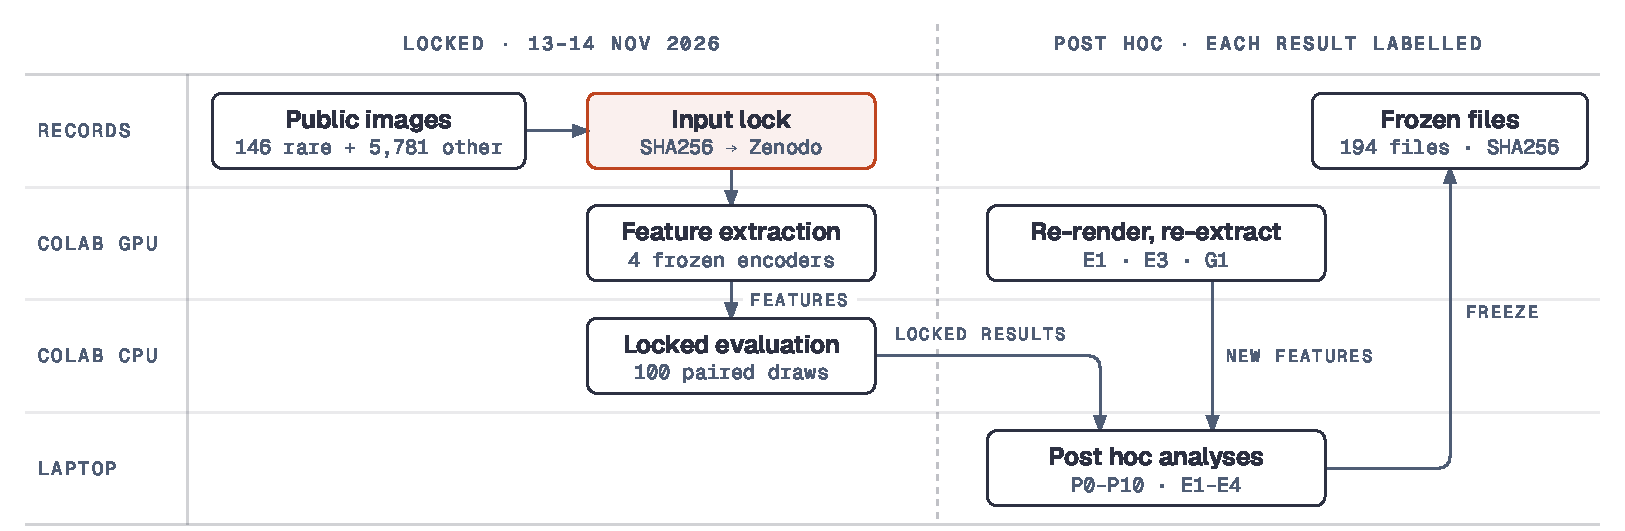
\includegraphics[width=\textwidth]{diagrams/pipeline.pdf}
\caption{How the study ran. Lanes: where each step ran, with the records (inputs, the hashed lock, the frozen files) in the top lane; left of the dashed line, the locked study (13--14 November 2026); right of it, the post hoc work, each result labelled with its rule's date (P0, P6 and P7 were computed before their rules; every other rule came first). Highlighted: the input lock, hashed before any score. P10's blind review was done by hand; every other step is a script or a notebook generated from one.}
\label{fig:pipeline}
% src: diagrams/pipeline.html (diagram-design skill, swimlane; exported by diagrams/export_pdf.py); counts ML l.166-170 and l.237;
%      dates ML l.142-144 and PR section 8 (S2-S4 rows); controls ML l.237-249; evaluation location PR l.150-151; P0, P6, P7 before their rules ML l.227
\end{figure*}

\section{Background and Phase 0}
\subsection{Frozen encoders and few-shot classification}
We compare four frozen encoders that differ in architecture, pretraining data and objective. \emph{Inception-v3} \cite{Szegedy2016} is a convolutional network trained with labels on ImageNet (2048-d features), the backbone family of Yoo et al. \emph{DINOv2} \cite{DINOv2} is a self-supervised vision transformer (ViT-B/14, 768-d) trained on natural images. \emph{RETFound} \cite{RETFound2023} is a ViT-L/16 pretrained on retinal images as a masked autoencoder \cite{He2022}, which learns by reconstructing hidden image patches; we use its OCT weights (1024-d). \emph{MIRAGE} \cite{MIRAGE2025} is a multimodal OCT foundation model pretrained with a masking objective on OCT, scanning-laser (SLO) and retinal-layer images; we use its Base model on OCT input only ($512\times512$ input, 768-d).
Nothing is fine-tuned. RETFound was pretrained partly on Kermany images, and MIRAGE's pretraining data include unlabelled scans of four of the five benchmark diseases; DINOv2 is web-trained and may have seen these pictures.
% src: architectures and pretraining: docs/research/FM_FEWSHOT_PLAN.md l.275-277 (RETFound-MAE ViT-L/16, DINOv2 ViT-B/14, MIRAGE-Base 512x512 patch 32) and LITERATURE_KB.md A02-A04; feature sizes and exposure ML l.178, 184

The classifier is a cosine prototype, as in SimpleShot \cite{SimpleShot2019} without its centring step: L2-normalise each support feature, average per class, normalise again, and assign each query to the closest prototype. The metric is macro recall, the mean of per-class recall (chance 0.20 for five classes).
% src: ML l.192, 194

\subsection{Acquisition cues in the images}
Image sizes differ by class (Fig.~\ref{fig:sizes}). Every encoder resizes its input to a fixed size, and DINOv2 and RETFound also centre-crop it, keeping a median 0.69--0.77 of each benchmark image. Resizing changes the pixel count but keeps the layout of the image, including the dark bands around the scan: among development images, the median share of the image in flat border rows and columns is 0.34--0.50 per rare class, against at most 0.002 for every Kermany, OCTID and OCTDL class. Whether any model uses these cues was not tested.
% src: ML l.490 (resizing keeps the layout; cues not tested; aspect-ratio clause dropped, claim ledger D15); crop share ML l.180; border share ML l.160 (development images, locked geometry summary)

\begin{figure}[t]
\centering
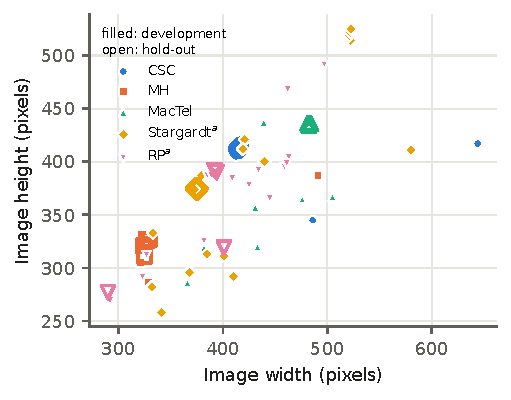
\includegraphics[width=0.86\columnwidth]{figures/fig3_image_sizes.pdf}
\caption{Width and height of the 146 benchmark rare images, from the input lock. Filled: the 124 development images; open: the 22 hold-out images. Image size differs by class; the size-only reference uses only these two numbers. \fnRS The folder labels for RP and Stargardt disagree with the counts in the original paper.}
\label{fig:sizes}
% src: LOCK image_inventory.csv columns label, split, width, height (as ML fig:sizes)
\end{figure}

\begin{table*}[t]
\caption{Development five-way macro recall (primary, locked): 124 queries, five folds pooled; mean over 100 support draws per $K$, every model on the same supports and queries.}
\label{tab:dev}
\centering\footnotesize
\resizebox{\textwidth}{!}{% src: means ARC reports/nomination/nomination.json arms.<arm>.k_scores and .score (locked);
% src: SD and 5th-95th of arm and paired rows: PH R2_development_spread.csv (rule R2, commit 65fe98c,
%      computed 2026-11-20 after the results were known; gate: R2 means equal nomination.json within 1e-9);
%      paired means: R2 'X minus Inception' rows; size-only: ARC reports/legacy/size_only_reference.csv lines 2-6.
\begin{tabular}{@{}lccccc@{}}
\toprule
Arm & $K=1$ & $K=2$ & $K=4$ & $K=8$ & Mean $K$ 1--8 \\
\midrule
MIRAGE (nominee) & \makecell{0.495\\{\scriptsize (0.046)$^\dagger$}} & \makecell{0.615\\{\scriptsize (0.048)$^\dagger$}} & \makecell{0.712\\{\scriptsize (0.040)$^\dagger$}} & \makecell{0.777\\{\scriptsize (0.030)$^\dagger$}} & \makecell{0.650\\{\scriptsize (0.028; 0.603--0.688)$^\dagger$}} \\
DINOv2 & \makecell{0.407\\{\scriptsize (0.046)$^\dagger$}} & \makecell{0.497\\{\scriptsize (0.043)$^\dagger$}} & \makecell{0.616\\{\scriptsize (0.043)$^\dagger$}} & \makecell{0.711\\{\scriptsize (0.031)$^\dagger$}} & \makecell{0.558\\{\scriptsize (0.028; 0.511--0.606)$^\dagger$}} \\
Inception-v3 (reference) & \makecell{0.409\\{\scriptsize (0.046)$^\dagger$}} & \makecell{0.499\\{\scriptsize (0.043)$^\dagger$}} & \makecell{0.581\\{\scriptsize (0.039)$^\dagger$}} & \makecell{0.647\\{\scriptsize (0.033)$^\dagger$}} & \makecell{0.534\\{\scriptsize (0.029; 0.494--0.583)$^\dagger$}} \\
RETFound & \makecell{0.318\\{\scriptsize (0.040)$^\dagger$}} & \makecell{0.375\\{\scriptsize (0.041)$^\dagger$}} & \makecell{0.442\\{\scriptsize (0.039)$^\dagger$}} & \makecell{0.489\\{\scriptsize (0.031)$^\dagger$}} & \makecell{0.406\\{\scriptsize (0.024; 0.367--0.441)$^\dagger$}} \\
\midrule
\makecell[l]{MIRAGE $-$\\Inception-v3 (paired)} & \makecell{+0.086\\{\scriptsize (0.057; +0.001 to +0.184)$^\dagger$}} & \makecell{+0.116\\{\scriptsize (0.063; +0.015 to +0.230)$^\dagger$}} & \makecell{+0.132\\{\scriptsize (0.054; +0.052 to +0.222)$^\dagger$}} & \makecell{+0.130\\{\scriptsize (0.043; +0.071 to +0.210)$^\dagger$}} & \makecell{+0.116\\{\scriptsize (0.037; +0.069 to +0.185)$^\dagger$}} \\
\makecell[l]{DINOv2 $-$\\Inception-v3 (paired)} & \makecell{$-$0.002\\{\scriptsize (0.053; $-$0.089 to +0.077)$^\dagger$}} & \makecell{$-$0.002\\{\scriptsize (0.055; $-$0.094 to +0.087)$^\dagger$}} & \makecell{+0.036\\{\scriptsize (0.053; $-$0.046 to +0.120)$^\dagger$}} & \makecell{+0.064\\{\scriptsize (0.042; $-$0.008 to +0.136)$^\dagger$}} & \makecell{+0.024\\{\scriptsize (0.034; $-$0.025 to +0.086)$^\dagger$}} \\
\makecell[l]{RETFound $-$\\Inception-v3 (paired)} & \makecell{$-$0.090\\{\scriptsize (0.057; $-$0.182 to $-$0.000)$^\dagger$}} & \makecell{$-$0.124\\{\scriptsize (0.059; $-$0.231 to $-$0.029)$^\dagger$}} & \makecell{$-$0.139\\{\scriptsize (0.049; $-$0.217 to $-$0.060)$^\dagger$}} & \makecell{$-$0.159\\{\scriptsize (0.044; $-$0.232 to $-$0.086)$^\dagger$}} & \makecell{$-$0.128\\{\scriptsize (0.035; $-$0.186 to $-$0.070)$^\dagger$}} \\
\midrule
Size-only reference & \makecell{0.578\\{\scriptsize (0.058)}} & \makecell{0.550\\{\scriptsize (0.052)}} & \makecell{0.560\\{\scriptsize (0.051)}} & \makecell{0.589\\{\scriptsize (0.049)}} & \makecell{0.569\\{\scriptsize (0.036; 0.508--0.619)}} \\
Chance & 0.200 & 0.200 & 0.200 & 0.200 & 0.200 \\
\bottomrule
\end{tabular}
}
\par\smallskip
\parbox{\textwidth}{\footnotesize Cells: mean; below it, SD and 5th--95th percentiles over draws (rule R2). These describe variation over support draws for these images; they are not confidence intervals. Paired rows: difference from Inception-v3 on the same draws. $^\dagger$Pre-specified quantity computed after the results were known (rule R2, 19--20 November 2026); every mean equals the locked value. Chance is 0.20. MIRAGE was nominated; no other model was within 0.02.}
\end{table*}

\subsection{Phase 0: replication of Yoo et al.}
We first rebuilt the pipeline of Yoo et al.\ from the public data: a fixed split manifest; basic augmentation; one CycleGAN \cite{Zhu2017} per rare disease that translates normal B-scans into that disease (100 epochs, 4,000 images generated per disease); an automatic quality filter in Inception-v3 feature space in place of the paper's ophthalmologists, which kept 832 to 3,000 images per class; and a nine-class Inception-v3 with frozen convolutional layers and a trained softmax layer. At seed 42 the CycleGAN variant reached 92.95\% accuracy on our 1,022 test images (the paper reports 92.1\% on its own test, whose images are not public: context, not a like-for-like comparison), against 90.31\% with real images only and 88.85\% with basic augmentation. Over five training seeds, however, CycleGAN ($92.59\pm1.29$\%) and basic augmentation ($92.93\pm1.85$\%) were not separated; both named 17--19 of the 22 rare test images correctly, against 11--17 with real images only. Rare and common images were also almost linearly separable in frozen Inception-v3 features, so disease and source were confounded. These results motivated Phase~1: no generated images, frozen encoders, and controls for the source.
% src: README at 6116f93 (Results; results/stage4/metrics.csv, results/seed_check.csv); QC kept counts docs/research/REPLICATION.md l.286 (3,000/2,610/1,248/2,199/832); 100 epochs, 4,000 generated each README Status table; context ML l.123; separability ML l.91 (C0, AUC 0.995 to 0.991 README Status)

\section{Implementation}
Fig.~\ref{fig:pipeline} shows the pipeline. \textbf{Data.} The 146 rare images; 4,000 Kermany images for fitting the nine-way head (1,000 per class) and its 1,000 official test images; and, as queries only, OCTID (206 normal, 102 CSC, 102 MH) \cite{OCTID2020} and OCTDL (332 normal scans from 110 patients, 39 MH) \cite{OCTDL2024}.
\textbf{Input lock.} Rosters, episode draws, model identities, code and rules were hashed (SHA256) into an input lock on 13 November 2026, and the hashes are on Zenodo (doi:10.5281/zenodo.24206472); the lock's approval was recorded before the first score.
\textbf{Feature extraction} ran on one NVIDIA L4 GPU in Google Colab. Each encoder uses the input transform of its own published code: MIRAGE resizes to $512\times512$, converts to grey and min--max scales; Inception-v3 resizes to 256 then 299; DINOv2 and RETFound resize and centre-crop. Median warm time was 13.57 (MIRAGE), 14.03 (DINOv2), 23.91 (RETFound) and 323.66\,ms per image (Inception-v3). Before the lock, each model's outputs from two timed passes had to agree to a cosine of at least 0.9999; all four passed on the first attempt.
\textbf{Evaluation.} The locked evaluation ran in a second Colab notebook on a CPU runtime, from the cached features and the locked episodes: cosine prototypes, a secondary logistic probe, the size-only reference, the nomination and every report. Most post hoc analyses ran on a laptop from the same files; the \textbf{controls} that need new features re-render images and re-extract them on the GPU; unchanged originals passed through the locked extraction must reproduce the locked features to within $10^{-4}$ of the largest output.
\textbf{Engineering details.} RETFound's checkpoint loads with missing keys for its final normalisation and head and 106 unexpected keys; as in the upstream frozen-feature code, we keep its default, untrained final LayerNorm. The locked duplicate screen fingerprinted identical files, identical pixels and a 64-bit difference hash (Hamming distance at most 4); it flagged no pair, yet a post hoc keypoint screen and blind review (P10) later found 14 same-picture pairs.
% src: RETFound keys supplement S5 note (DRV step11_pilots.txt) and ML l.182; duplicate screen ML l.163 and P10 ML l.375
\textbf{Software.} 17 Python modules for the two pipelines (11,227 lines) and 318 unit tests in the repository; the Colab notebooks are generated from the scripts and pinned to commits; every table and figure is generated from the result files.
% src: evaluation location PR l.150-151 (steps 6-8 in colab_fm_evaluate.ipynb, CPU), laptop post hoc ML l.227; data ML l.166-170; lock and Zenodo ML l.142-144; transforms ML l.180; timings and repeat check supplement S5 tab:pilot (DRV step11_pilots.txt: 13.57, 14.03, 323.66, 23.91 ms) and ML l.186; control check ML l.237; software: wc -l fm_*.py stage*.py (17 files, 11,227 lines) and 318 "def test_" in tests/*.py and test_analysis_cluster.py, at commit a9ad899

\section{Experimental Design and Controls}
\textbf{Development.} The 124 development images (CSC 27, MH 26, MacTel 25, Stargardt 19, RP 27) were dealt into five fixed folds; the images carry no patient IDs, so folds are image-level. For each held-out fold, $K=1$, 2, 4 and 8 supports per class were drawn from the other folds, 100 times, nested across $K$. Every model saw exactly the same supports and queries, so differences between models are paired by draw. Where one number is needed it is the mean over $K=1$, 2, 4, 8.
% src: ML l.150, l.190
\textbf{Nomination.} One foundation model was nominated from the development folds only (models within 0.02 of the best tie; the fastest wins) and sealed before any hold-out or external image was scored.
% src: ML l.198
\textbf{Hold-out.} 22 images (5 CSC, 5 MH, 4 MacTel, 4 Stargardt, 4 RP), drawn once with a fixed seed; supports come from all 124 development images. They were inspected in our earlier work, so the test is not blind and we read it for direction only.
% src: ML l.152
\textbf{Nine-way audit.} Adding the four Kermany classes, we count normal scans that the head calls any rare class (\emph{false rare}), per source: 169 Kermany normal test images whose patients appear in no fitting row, 206 from OCTID and 332 from OCTDL. Beside each rate we show the share of the same sources' disease images called rare (R1, post hoc), because a low false-rare rate can also mean that the head rarely says ``rare''.
% src: ML l.166, l.229
\textbf{Exploratory.} OCTID CSC against MH, with benchmark supports. We evaluated agreement with OCTID's and OCTDL's published CSC/CSR and MH labels using benchmark-only $K$-shot supports. Clinical label equivalence, patient independence and freedom from acquisition shortcuts were not established.
% src: required wording AM l.47-49 (A1 rule 7), as printed at ML l.171

\begin{table*}[t]
\caption{Nine-way audit (locked; R1 post hoc): truly normal scans that the head calls any of the five rare classes, with called-NORMAL counts and, beside them, disease images of the same sources called rare.}
\label{tab:frr}
\centering\footnotesize
\resizebox{\textwidth}{!}{% src: ARC reports/external/external_source_audit.csv (numerator, value, interval_low, interval_high);
%      Kermany 169 = false_rare_rate_patient_disjoint, Kermany 250 = false_rare_rate_all, OCTID/OCTDL = false_rare_rate;
%      called NORMAL = recall_NORMAL numerators; R1 (post hoc) = PH R1_rare_beside_false_rare.csv rare_called_any_rare.
\begin{tabular}{@{}lcccccc@{}}
\toprule
 & \multicolumn{4}{c}{Normal scans called any rare class: count (rate; 95\% interval)} & Called NORMAL & R1$^\ddagger$: disease images called any rare \\
\cmidrule(lr){2-5}
Arm & \makecell{Kermany, of 169\\(headline)} & \makecell{Kermany, of 250\\(secondary)} & OCTID, of 206 & OCTDL, of 332 & OCTID / OCTDL & \makecell{OCTID CSC / MH (of 102);\\OCTDL MH (of 39)} \\
\midrule
MIRAGE & \makecell{0\\{\scriptsize (0.000; 0.000--0.000)}} & \makecell{0\\{\scriptsize (0.000; 0.000--0.000)}} & \makecell{4\\{\scriptsize (0.019; 0.005--0.049)}} & \makecell{30\\{\scriptsize (0.090; 0.055--0.136)}} & 202 / 26 & 41 / 11; 3 \\
DINOv2 & \makecell{6\\{\scriptsize (0.036; 0.012--0.065)}} & \makecell{10\\{\scriptsize (0.040; 0.017--0.066)}} & \makecell{17\\{\scriptsize (0.083; 0.049--0.129)}} & \makecell{141\\{\scriptsize (0.425; 0.372--0.472)}} & 188 / 145 & 69 / 85; 39 \\
Inception-v3 & \makecell{4\\{\scriptsize (0.024; 0.006--0.049)}} & \makecell{7\\{\scriptsize (0.028; 0.008--0.053)}} & \makecell{15\\{\scriptsize (0.073; 0.041--0.117)}} & \makecell{11\\{\scriptsize (0.033; 0.012--0.059)}} & 182 / 66 & 46 / 44; 1 \\
RETFound & \makecell{1\\{\scriptsize (0.006; 0.000--0.019)}} & \makecell{1\\{\scriptsize (0.004; 0.000--0.013)}} & \makecell{0\\{\scriptsize (0.000; 0.000--0.018)}} & \makecell{18\\{\scriptsize (0.054; 0.029--0.087)}} & 189 / 137 & 0 / 0; 3 \\
\bottomrule
\end{tabular}
}
\par\smallskip
\parbox{\textwidth}{\footnotesize Kermany headline: the 169 normal test images whose patients are in no fitting row. Intervals: cluster resamples by patient (Kermany) or dependence group (OCTDL); exact Clopper--Pearson for OCTID. $^\ddagger$R1 is post hoc.}
\end{table*}

\begin{table}[t]
\caption{Hold-out (locked, secondary) and OCTID two-way (locked, exploratory).}
\label{tab:holdout}
\centering\footnotesize
\setlength{\tabcolsep}{2.2pt}
\resizebox{\columnwidth}{!}{%
\begin{tabular}{@{}lcccccccc@{}}
\toprule
 & \multicolumn{6}{c}{Nine-way: named correctly} & \makecell{Hold-out\\five-way} & \makecell{OCTID\\CSC/MH} \\
\cmidrule(lr){2-7}
Model & CSC & MH & MacTel & Starg.\fnRS & RP\fnRS & \textbf{of 22} & \multicolumn{2}{c}{mean over $K$ (SD)} \\
\midrule
MIRAGE & 5 & 5 & 2 & 4 & 4 & \textbf{20} & 0.722 (0.063) & 0.737 (0.069) \\
DINOv2 & 4 & 4 & 4 & 2 & 1 & \textbf{15} & 0.526 (0.065) & 0.768 (0.058) \\
Inception-v3 & 4 & 4 & 1 & 3 & 1 & \textbf{13} & 0.524 (0.067) & 0.711 (0.051) \\
RETFound & 1 & 1 & 2 & 1 & 4 & \textbf{9} & 0.338 (0.065) & 0.512 (0.027) \\
Size-only & -- & -- & -- & -- & -- & -- & 0.618 (0.101) & 0.500 (0.000) \\
\bottomrule
\end{tabular}}
\par\smallskip
\parbox{\columnwidth}{\footnotesize Class sizes 5, 5, 4, 4, 4; the hold-out is read for direction only. Five-way chance 0.20; two-way chance 0.50. Spreads over 100 support draws. \fnRS The folder labels for RP and Stargardt disagree with the counts in the original paper.}
% src: nine-way counts and hold-out means/SD tables/t3_holdout.tex (frozen); OCTID means/SD tables/t4_octid_two_way.tex (frozen)
\end{table}

\begin{table*}[t]
\caption{Post hoc E1 (rule committed 20 Nov 2026): MIRAGE minus Inception-v3, development macro recall averaged over $K$ within each of 100 paired draws, per feature set, with the companion lines.}
\label{tab:e1d}
\centering\footnotesize
% src: E1d_success.csv in results/fm_v1/posthoc (generated by make_tables.py; formatting only);
% label: post hoc, Phase-1 rule E1 timestamped by commit 4b4e883 (20 Nov 2026), computed 2026-11-21; outside the locked protocol; never replaces a locked result; limitations: the centre square drops lateral retina unequally by source and class; MIRAGE now gets 256 px of detail enlarged to 512; E1-M does not remove effective resolution (content short side 103-496 px), field of view, scanner appearance, compression, intensity, black-clipped background against speckle, or Kermany's white fill wedges
% cells: n_draws, mean, sd, p05 (four decimals), draws_above_0, verdict as stored; mean and p05 are paired differences.
\begin{tabular}{@{}p{4.4cm}lp{2.2cm}cccccl@{}}
\toprule
Line & Feature set & Status & $n$ & Mean & SD & p05 & Draws $>0$ & Verdict \\
\midrule
MIRAGE $-$ Inception-v3 & locked & interpreted & 100 & +0.116 & 0.037 & +0.0689 & 100 & description only \\
MIRAGE $-$ Inception-v3 & E1-M & interpreted & 100 & +0.063 & 0.036 & +0.0025 & 95 & pass \\
MIRAGE $-$ Inception-v3 & E1-L & interpreted & 100 & +0.077 & 0.034 & +0.0229 & 99 & description only \\
MIRAGE $-$ Inception-v3 & E1-C & interpreted & 100 & +0.068 & 0.033 & +0.0167 & 98 & description only \\
MIRAGE E1-M $-$ Content-size reference (raw content box) & E1-M & interpreted & 100 & +0.203 & -- & +0.1493 & 100 & companion line \\
MIRAGE E1-M $-$ Thumbnail reference (E1-M) & E1-M & interpreted & 100 & +0.290 & -- & +0.2427 & 100 & companion line \\
\bottomrule
\end{tabular}

\par\smallskip
\parbox{\textwidth}{\footnotesize Only the E1-M row gives the verdict ($p_{05}>0$); the other rows are descriptions. Limitations stated with every E1 result: the centre square drops lateral retina unequally by source and class; MIRAGE now gets 256 px of detail enlarged to 512; E1-M does not remove effective resolution (content short side 103-496 px), field of view, scanner appearance, compression, intensity, black-clipped background against speckle, or Kermany's white fill wedges.
 (Correction: the measured content short side of the 146 rare images is 103--471\,px.) Label: post hoc, Phase-1 rule E1 timestamped by commit 4b4e883 (20 Nov 2026), computed 2026-11-21; outside the locked protocol; never replaces a locked result
.}
\end{table*}

\textbf{References without a model.} The \emph{size-only} rule assigns each query to the class whose supports have the nearest mean width and height; it was registered with the protocol. A $16\times16$ grey thumbnail with the same nearest-mean rule is a post hoc pixel reference.
% src: ML l.240 (references), PR A2 N-1
\textbf{Post hoc controls.} After the locked results, we committed four further rules on 20 November 2026, before any of their numbers. \emph{E1}, a size and framing control: every image is cropped to its content box, cut to the centred square and resized to $256\times256$ once for all models; it passes if the 5th percentile over the 100 paired draws of MIRAGE minus Inception-v3 (each draw averaged over $K$) is above 0, that is, if at most four draws are non-positive; with six or more it fails. \emph{E2} analyses where external normal scans go. \emph{E3} varies the preprocessing of MIRAGE and RETFound. \emph{E4} is a few-shot source test: two-way prototypes that tell normal scans of two sources apart (chance 0.50). A same-picture audit (\emph{P10}: keypoint screen and blind review) looked for duplicates the locked screen missed. Every post hoc result is labelled and never replaces a locked one.
% src: ML l.237-249 (E1-E4 rules), l.375 (P10)

\section{Results}
\subsection{Locked results}
Table~\ref{tab:dev} gives the primary result. MIRAGE was nominated: its development macro recall was the highest at every $K$, 0.650 on the mean over $K$, against 0.534 for Inception-v3; on the same draws it led by $+0.116$ (5th--95th percentile $+0.069$ to $+0.185$). But image size alone scored 0.578 at $K=1$, a higher mean than every model; MIRAGE's mean was higher only from $K=2$ (unpaired means). RETFound stayed below the size-only reference at every $K$; DINOv2 and Inception-v3 passed it only at $K=4$ and 8.
% src: ML l.114 and l.470 (Table I, ARC nomination.json, R2, size_only_reference.csv)

Table~\ref{tab:frr} counts false rares. With its locked recipe on the published, frame-filling inputs, MIRAGE called 0 of 169 patient-disjoint Kermany normal scans rare, 4 of 206 OCTID and 30 of 332 OCTDL; DINOv2 called 141 of the 332 OCTDL scans rare. A low false-rare rate can also mean that the head rarely says ``rare'': MIRAGE called only 26 of the 332 OCTDL normal scans normal, and 41 of 102 OCTID CSC, 11 of 102 OCTID MH and 3 of 39 OCTDL MH images any rare class (R1, post hoc).
% src: ML l.116 (MIRAGE counts, R1 41/11/3, 26 of 332); DINOv2 141 tables/t2_false_rare.tex
On the 22 hold-out images (Table~\ref{tab:holdout}), the nine-way head named 20 correctly for MIRAGE and 13 for Inception-v3; on the five-way task MIRAGE reached 0.722 on the mean over $K$, against 0.524 for Inception-v3 and 0.618 for the size-only reference. With four or five images per class, these show direction only. In the exploratory OCTID test, DINOv2 had the highest mean (0.768); MIRAGE reached 0.737 and RETFound collapsed to one class in up to 60 of 100 draws. These are agreement with published labels only; label equivalence, patient independence and freedom from acquisition shortcuts were not established.
% src: ML l.316 and tables/t3_holdout.tex; OCTID ML l.335 and tables/t4_octid_two_way.tex

\subsection{Post hoc controls}
\textbf{E1, size and framing (Table~\ref{tab:e1d}).} Under the size and framing control, MIRAGE keeps a positive development advantage over Inception-v3 (mean 0.063, locked 0.116; p05 0.003), and also when effective resolution is evened out (E1-L p05 = 0.023), and also when the image is only cropped to its content box (E1-C p05 = 0.017); it is above the pixel-only reference (mean 0.290). The margin is small: the 5th percentile is 0.0025, with 95 of the 100 draws above 0, so a sixth non-positive draw would have failed the rule. MIRAGE's own score barely moved (0.650 to 0.649), while Inception-v3 rose from 0.534 to 0.586 under the new input path.
% src: fixed sentence verbatim from PH E1_comparison.md "Sentence" (l.20); margin, 0.649 and 0.586 ML l.405 (PH E1d_success.csv, E1b_development.csv)

\textbf{False rares depend on the input recipe (post hoc).} Under E1's controlled inputs, MIRAGE called 261 of the 332 OCTDL normal scans rare (locked: 30), and within E3's preprocessing grid 10 of 20 external false-rare counts fell outside their model's locked 95\% interval, in both directions. Padding images to a square instead of stretching them (G1, post hoc) left MIRAGE calling 0 of 206 OCTID normal scans normal, against 202 unpadded. The locked false-rare rates therefore hold for each model's locked recipe on the published, frame-filling inputs, and we assign no cause.
\textbf{Preprocessing (E3).} MIRAGE stayed ahead of locked Inception-v3 in every variant of its grid (5th percentiles 0.043 to 0.075), but one normalisation constant moved RETFound from 0.406 to 0.578.
\textbf{Source (E4).} A few-shot test told normal scans of Kermany, OCTID and OCTDL apart above chance at every $K$ (two-way macro recall at least 0.67 at $K=1$; chance 0.50). On the mean over $K$ it ranged from 0.779 to 0.996 across models and inputs, and a $16\times16$ grey thumbnail alone reached 0.820 to 0.923: the source is visible in a handful of images, with or without a model. E4 does not show whether the models use the source in the rare-disease task.
\textbf{Duplicates (P10).} Four of the 22 hold-out images have a same-picture copy among the development images, which the locked screen did not flag. E1-D, post hoc, a rule added after the E1 verdict that excludes the 14 same-picture pairs and one same-case pair: ``Without the same-picture pairs, MIRAGE's development lead over Inception-v3 under E1-M has mean 0.064 and 5th percentile 0.0062 (with them: 0.063 and 0.0025).''
% src: E1g ML l.411 (261 of 332, locked 30); E3 ML l.417 (10 of 20; MIRAGE 0.043-0.075; RETFound 0.406 -> 0.578); G1 ML l.295 (PH G1_pad_to_square.csv: 202 -> 0); E4 ML l.63 (abstract) and ML l.420 (PH E4a_fewshot_source_test.csv: 0.7791-0.9964; thumbnails 0.8197-0.9230); P10 ML l.375 and E1-D ML l.408 (PH E1D_duplicate_sensitivity.csv)

\section{Discussion}
Each control changed how the locked numbers read. Beside the size-only reference, no model beat a rule that sees no pixel at one shot, and a model at or below that reference has not shown that it reads the retina. Beside R1, a low false-rare count can also mean that the head rarely says ``rare'', and the post hoc E1 inputs moved MIRAGE's OCTDL count from 30 to 261. Under the post hoc size and framing control, MIRAGE's lead (mean 0.063) held with no draw to spare. The post hoc source test showed that the sources are easy to tell apart, even from thumbnails; whether any model uses the source in the rare-disease task was not tested. For computer-vision practice: on a benchmark assembled from several sources, run model-free references and source tests beside every model, report false-rare rates per input recipe with R1, and audit duplicates with more than a perceptual hash.
% src: numbers as in Results above (ML l.114, l.116, l.405, l.411, l.420); reference reading ML l.99 (contribution 1); E4 reading ML l.527

\section{Limitations}
The images are web-collected and the labels are the published ones, not re-read by a clinician for this study, and the RP and Stargardt folder counts disagree with the original paper. The rare images have no patient IDs, so folds are image-level and same-patient leakage is unknown; P10 found copies across development and hold-out. The hold-out has four or five images per class and was inspected before. E1 is one control fixed in advance; its pass rests on the draws around the 5th percentile, whose own uncertainty was not estimated, and E1-M leaves effective resolution, field of view and scanner appearance in place. E1-D, post hoc: ``Without the same-picture pairs, MIRAGE's development lead over Inception-v3 under E1-M has mean 0.064 and 5th percentile 0.0062 (with them: 0.063 and 0.0025).'' Every post hoc result was computed after the locked results were known, and the audit framing was adopted after them. We tested frozen encoders only, at Base size for MIRAGE and DINOv2, with no fine-tuning. In Phase~0, the Kermany test split shares 566 of its 633 patients with the training pool.
% src: ML l.150-156, l.163, l.405, l.556 and tables/e1_limitations.tex; Phase 0 patients README at 6116f93 (results/analysis/cluster_summary.csv)

\section{Reproducibility}
The protocol, its three dated amendments and the input-lock hashes are on Zenodo (doi:10.5281/zenodo.24206472); all were hashed before any score. The locked code is commit \texttt{2f48654}, and the Colab notebooks are generated from the scripts and pinned to commits. 194 result, table and figure files are frozen in a SHA256 manifest that the unit tests check; rebuilding every table and figure reproduces them byte for byte. Code: \url{https://github.com/Malnoad/Few-shot-rare-diseases}. The data are public and not redistributed \cite{Kermany2018,Yoo2021,OCTID2020,OCTDL2024}.
% src: ML l.571-579 (data and code availability); freeze: results/fm_v1/phase1_freeze.json (194 files), protocols.md change log 26-27 Nov

\section{Conclusion}
Image size alone beat every frozen model at one shot on this benchmark, and each post hoc control changed how the model ranking reads. Few-shot rankings on multi-source benchmarks should be read beside size, framing and source controls, and false-rare rates per input recipe.
% src: ML l.567 (conclusion)

\section*{Acknowledgment}
During the preparation of this work the authors used AI assistants to help write code, check numbers and edit the text. The authors reviewed all content and take full responsibility for it.
% Placement: IEEE author policy, AI-generated content is disclosed in the acknowledgments section and the AI system is named
% (journals.ieeeauthorcenter.ieee.org, submission and peer review policies, read 27 Nov 2026); wording after Elsevier's
% declaration template ("During the preparation of this work the author(s) used ... in order to ..."; generative AI policies
% for journals, read 27 Nov 2026). Lam, 27 Nov: a small note only, without naming the assistants (IEEE's policy asks
% that the AI system be named; revisit if the report goes to an IEEE venue).

\bibliographystyle{IEEEtran}
\bibliography{references}
\end{document}
